%% This is file `DEMO-TUDaPub.tex' version 2.07 (2020/01/31),
%% it is part of
%% TUDa-CI -- Corporate Design for TU Darmstadt
%% ----------------------------------------------------------------------------
%%
%%  Copyright (C) 2018--2019 by Marei Peischl <marei@peitex.de>
%%
%% ============================================================================
%% This work may be distributed and/or modified under the
%% conditions of the LaTeX Project Public License, either version 1.3c
%% of this license or (at your option) any later version.
%% The latest version of this license is in
%% http://www.latex-project.org/lppl.txt
%% and version 1.3c or later is part of all distributions of LaTeX
%% version 2008/05/04 or later.
%%
%% This work has the LPPL maintenance status `maintained'.
%%
%% The Current Maintainers of this work are
%%   Marei Peischl <tuda-ci@peitex.de>
%%   Markus Lazanowski <latex@ce.tu-darmstadt.de>
%%
%% The development respository can be found at
%% https://github.com/tudace/tuda_latex_templates
%% Please use the issue tracker for feedback!
%%
%% ============================================================================
%%
% !TeX program = lualatex
%%

\documentclass[
	fontsize=10.5pt,
	marginpar=false,
	ngerman,
	accentcolor=3d
	]{tudapub}

\usepackage[english, main=ngerman]{babel}
\usepackage[babel]{csquotes}

\usepackage[
backend=biber,
style=alphabetic,
sorting=anyt
]{biblatex}
\bibliography{literature}

\usepackage{hologo}

\begin{document}

%Zusätzliche Metadaten für PDF/A. In diesem Fall notwendig, weil Titel ein Makro enthält.
\Metadata{
	author={Anna Stefanie Blümer, Tim Pollandt},
	title={Umgebungserkennung aus Rauschen},
	subject={Dokumentation zum Praktikum „Implementierung in Forensik und Mediensicherheit“},
	date=2021-02-26,
	keywords=TU Darmstadt \sep Praktikum \sep Fraunhofer \sep Forensik \sep Audio \sep Rauschen
}

\title{Umgebungserkennung aus Rauschen in Audiodaten}
\subtitle{Dokumentation zum Praktikum „Implementierung in Forensik und Mediensicherheit“}
\author{A. Stefanie Blümer, Tim Pollandt}

\titleimage{
%	%Folgende Box kann selbstverständlich durch ein mit \includegraphics geladenes Bild ersetzt werden.
	\color{TUDa-3d}\rule{\width}{\height}
}


%Varianten der Infoboxen
\addTitleBox{Prof. Martin Steinebach\\Dr.-Ing. Sascha Zmudzinski\\Fraunhofer SIT}
%\addTitleBoxLogo{example-image}
%\addTitleBoxLogo*{\includegraphics[width=.3\linewidth]{example-image}}



\maketitle

%\begin{abstract}
%	…
%\end{abstract}
%
%\begin{abstract}[english]
%	…
%\end{abstract}


%\pagebreak
\tableofcontents

\pagebreak
\IMRADlabel{introduction}
\section{Übersicht}
Hier werden wir kurz in die Thematik einführen und einen Überblick über die Teile des Projekts geben.

\subsection{Einführung}
In der Forensik ist es wichtig Manipulationen in Audiodaten erkennen zu können, um etwa Beweismittel auf ihre Plausibilität prüfen zu können. Darüber hinaus ist es sehr hilfreich prüfen zu können, ob Aufnahmen an einer bestimmten Stelle aufgenommen sein könnten. Dadurch ist es möglich qualitativ unzureichend gefälschte Aufnahmen zu erkennen.

Neben vielen weiteren Ansätzen wie etwa Hall oder ENF\footnote{Elektrische Netzfrequenz}-Muster kann hierzu das spezifische Rauschen eines Ortes genutzt werden. Dieses unterscheidet sich je nach Umgebung und enthält hohe Anteile unterschiedlicher Frequenzen, die verglichen werden können.

\subsection{Ansatz}

Unser Ansatz basiert auf der Arbeit von Ikram und Malik \cite{ikram_digital_2010}. Unser Ziel ist es durch Betrachtung des Rauschens einer Audiodatei zu beurteilen, ob diese an bestimmten Orten aufgenommen wurde. Dies kann einerseits zur Plausibilitätsprüfung behaupteter Aufnahmeorte genutzt werden, ermöglicht andererseits mit Erweiterungen auch verschiedene Ansätze zur Erkennung, ob in einer Audiodatei Abschnitte aus anderen, an einem anderen Ort aufgenommenen, Aufnahmen eingefügt wurden. Dadurch wären viele Manipulationen erkennbar.

Im Folgenden arbeiten wir meist im Frequenzraum, haben zunächst also eine Schnelle Fourier-Transformation (FFT) durchgeführt.

Da die Erkennung von Orten und Manipulationen auf Aufnahmen arbeiten soll, in denen Sprache vorhanden ist, müssen wir diese Sprachelemente zunächst eliminieren bzw. reduzieren, um reines Rauschen vergleichen zu können. Dieses Rauschen kann zwar über den zeitlichen Verlauf weiterhin variieren (etwa durch vorbeifahrende Autos), der Einfluss solcher Effekte kann allerdings durch verschiedene Parameter, wie etwa die Nutzung von Median/Mittelwert in verschiedenen Verarbeitungsschritten später beeinflusst werden. Um vorzubereiten, dass Manipulationen auch dann erkannt werden, wenn ausschließlich ein Sprachsegment, also ein Audioteil ohne reine Rauschsequenzen, inseriert wurden, kommt ein Herausschneiden aller Teile mit Sprache nicht infrage und wir müssen auch an diesen Stellen das reine Rauschen extrahieren.

Dazu nutzen wir einen zweistufigen Ansatz in dem zunächst eine Standard-Rauschreduzierung durchgeführt wird. Durch Subtraktion dieses sprachreduzierten Signals erhalten wir eine erste Rauschapproximation. In einer weiteren Stufe reduzieren wir anschließend weiter sogenannte Voice Leakage, also verbliebene Einflüsse von Sprache. Mehr Details zur Rauschreduzierung folgen in Abschnitt \ref{noiseremove}.

Anschließend folgt eine Zuordnung von Audiodateien zu verschiedenen Umgebungen. An dieser Stelle haben wir ein eigenes Vorgehen entwickelt, das auf Abweichungen zu einem erwarteten Rauschen basiert. Dazu nehmen wir zunächst zu verschiedenen Umgebungen jeweils einige Audiodateien als Grundlage. Diese müssen jeweils ein kurzes Intervall reinen Rauschens (also Sprachfreiheit) enthalten, um optimale Ergebnisse bei der Rauschreduzierung zu erzielen. Zur Erstellung des erwarteten Rauschens der jeweiligen Umgebung wird dann allerdings der gesamte Zeitraum genutzt, da überall die Sprache wie oben beschrieben entfernt wurde. Durch Segmentierung aller in einer Umgebung aufgenommenen Dateien haben wir nun viele Segmente aus denen wir die Rauscherwartung bestimmen. Mit den Rauscherwartungen verschiedener Umgebungen vergleichen wir später die Rauschapproximationen zuzuordnender Aufnahmen und können so Plausibilitäten abschätzen, dass diese in einer bestimmten Umgebung aufgenommen wurden. Details zu diesem Prozess und den Metrikvariationen werden in Abschnitt \ref{envdetect} beschrieben. Weitere Ansätze werden in Abschnitt \ref{future} beschrieben.

Derzeit ist die Software trotz der Schaffung vieler Grundlagen noch nicht voll für den Einsatz zur Erkennung von Manipulationen in Dateien geeignet. Nöte Schritte und Ideen dazu werden in Abschnitt \ref{manipulationdet} diskutiert.

\pagebreak
\section{Implementierung}
Im Folgenden gehen wir auf die Teile der Implementierung ein und wie diese funktionieren. Details zu den einzelnen Methoden sind im Quelltext dokumentiert und werden hier deshalb ausgelassen. Die Details zur Bedienung unserer Software sind im Abschnitt \ref{usage} zu finden. Auf die Ergebnisse und Grafiken aus der Software gehen wir in Abschnitt \ref{reults} ein. Details zu den generierbaren Plots folgen in den Abschnitten \ref{plots} und \ref{usage}.

\subsection{Allgemein}

Unsere Implementierung ist in Python geschrieben. Das ermöglicht die Nutzung effizienter Library-\linebreak Implementierungen von Funktionen wie etwa FFT aus NumPy und einfachen In- und Export sowie Verarbeitung von Audio-Signalen und strukturierten Daten wie CSV. Eine gute Alternative wäre eine Implementierung in der ebenfalls verbreiteten Sprache Matlab mit ähnlichen Eigenschaften.

Zunächst lesen wir Audiospuren aus WAV-Dateien als Signalvektor ein. Unsere Audiodateien sind zunächst mit einem Gerät und ohne Rauschunterdrückung bzw. Lautstärkeadaption aufgenommene WAV-Dateien mit einer Samplerate von 44,1kHz und einer Tonspur. Die Software funktioniert jedoch auch mit anderen Frequenzen und kann auch Stereo-Dateien einlesen, wobei die Analysen jedoch nur auf einer der Spuren ausgeführt werden.

Unsere vollständige Implementierung sowie eine Liste der benötigten pip-Pakete und ein Beispielskript zur Nutzung der Software sind unter \cite{blumer_polltip4fm_2020} zu finden. % TODO noch nicht öffentlich bzw. Skript nicht existent.

\IMRADlabel{methods}
\subsection{Rauschextraktion}
\label{noiseremove}

Wir analysieren zunächst auf kleinen Fenstern das Vorhandensein von Sprache. Dazu nutzen wir auf den Fenstern eine Implementierung von Googles WebRTCVAD \cite{wiseman_webrtcvad_nodate}. Diese ist grundlegend nur für wenige Samplerates implementiert. Deshalb approximieren wir das Resultat durch Nutzung der logarithmisch nächsten Samplerate, was in unseren Tests zu sehr guten Ergebnissen führte. Aus der booleschen Klassifizierung kleiner Fenster nach Enthalten von Sprach- bzw. Tonanteilen detektieren wir darauf basierend das größte Intervall mit reinem Rauschen in der gegebenen Audiodatei. Dieses wird benötigt, um eine Rauschreduzierung durchführen zu können. Die rauschreduzierte Version ist dann Grundlage für die Extraktion reinen Rauschens.

Mithilfe des zuvor bestimmten größten Rauschintervalls führen wir nun eine Rauschreduzierung auf überlappenden Fenstern durch. Diese ist ähnlich zur Implementierung in Audacity. Dennoch funktionierte sie – vermutlich durch flexiblere Parametrisierung und die automatische Erkennung eines geeigneten Rauschintervalls – besser\footnote{Auch wenn es hier keine klare Metrik gibt, basiert diese Aussage auf einem akustischen Anhören der resultierenden Audiodateien und der Betrachtung von Zeit-Frequenz-Plots in denen die jeweiligen Energien durch Farben dargestellt werden. Jeweils kann das Verbleiben von Sprachfrequenzen subjektiv beurteilt werden.}. Eine erste Rauschapproximation erhalten wir nun durch Subtraktion des rauschreduzierten Signals vom Ursprungssignal.

Um verbleibende Sprachanteile „Voice Leakage“ weiter zu reduzieren, folgen wir dem Ansatz von \cite{kamath_multi-band_2002}. Dort wird Multiband Spectral Subtraction vorgestellt, durch die frequenzbandspezifisch Sprachanteile im Rauschen und zuvor zu stark reduziertes Rauschen ausgeglichen werden. Die Formeln lassen wir hier aus und verweisen auf das o.~g. Paper sowie den Quellcode. Unter Zuhilfenahme einer Matlab-Implementierung \cite{zavarehei_multi-band_nodate} haben wir eine funktionell an unsere Bedürfnisse angepasste Python-Implementierung erstellt. Diese nutzt in unserer angepassten Version die zuvor erkannten Intervalle reinen Rauschens als Grundlage. Hierbei mussten wir zwar einen deutlichen Abfall der Gesamtenergie und damit einen potenziellen Präzisionsverlust verzeichnen, erhielten aber nach o.~g. Kriterien auch sprachfreiere Ergebnisse.

Zu beachten ist, dass auch in der Implementierung der Multiband Spectral Subtraction ein Voice Activity Detector~(VAD) zwecks Sprachklassifizierung zum Einsatz kommt. Im Gegensatz zum zuvor erwähnten, basiert dieser jedoch darauf bereits ein kurzes Intervall reinen Rauschens als Grundlage zu haben und bekommt somit bei uns auch das längste Rauschintervall aus der Klassifizierung vor der ersten Rauschreduzierung.

\pagebreak
\subsection{Umgebungsdetektion}
\label{envdetect}

Um das Rauschen verschiedener Aufnahmen verschiedenen Umgebungen zuzuordnen bzw. Zuordnungsplausibilität zu prüfen, vergleichen wir die Energieabweichungen aller Frequenzen zwischen Umgebungsrauschen und Rauschen der Aufnahme.

Zunächst generieren wir also pro Umgebung eine erwartete Energie pro Frequenz. Dazu berechnen wir den Median aus allen Fenstern (Länge unterschiedlich wählbar) aller an diesem Ort aufgenommenen Aufnahmen.

Zur Zuordnung bzw. Plausibilitätsprüfung berechnen wir den Median der Frequenzenergien nun also auch über die Fenster einer Aufnahme. Damit können wir nun durch verschiedene Abweichungsberechnungen verschiedene Metriken erhalten. Grundlegend mitteln wir die quadrierten Abweichungen aller Frequenzen und sehen Umgebungen mit kleineren Ergebnissen als plausibler an. Implementierte Metrikänderungen sind die folgenden:
\begin{itemize}
	\item Lineare (oder andere wie Wurzel) Abweichungsberechnung statt quadrierter Abweichungsberechnung
	\begin{itemize}
		\item gewichtet einzelne starke Abweichungen weniger extrem
		\item funktionierte in Tests schlechter
	\end{itemize}
	\item Logarithmische y-Skalierung vor Differenzberechnung und anschließende Anwendung der Exponentialfunktion
auf die Differenzen
	\begin{itemize}
		\item betrachtet prozentuale statt absoluten Abweichungen
		\item beides ähnlich gut, abhängig von anderen Parametern
	\end{itemize}
	\item Mean oder Median für Differenzen
	\begin{itemize}
		\item derzeit: Mean über Differenzen eines Fensters, um starke Abweichungen in ein paar Frequenzen nicht zu vernachlässigen
		\item derzeit: Median über die Fenster einer Aufnahme, um einzelne Signalstörungen (bspw. herunterfallende Gegenstände) zu vernachlässigen
	\end{itemize}
	\item Gewichtungen der Frequenzen (x-Achse)
	\begin{itemize}
		\item gleichverteilt (Standard) → funktioniert gut
		\item Bevorzugung niedriger Frequenzen, da dort nach FFT geringe Frequenzdichte pro Oktave → funktioniert gut
		\item geringere Gewichtung des Sprachspektrums (implementiert durch zwei Gauß-Kurven) → funktioniert weniger gut
	\end{itemize}
\end{itemize}


\subsection{Empfehlungen}
Aktuell akzeptiert die Implementierung ausschließlich WAV-Dateien. Diese können mit verschiedenen Frequenzen erstellt werden, bei Stereo-Dateien geschieht die Analyse derzeit ausschließlich auf der linken Audio-Spur. Aufgrund der Implementierungen genutzter Frameworks gibt es zwar feste Frequenzen, auf denen die Klassifierung von Segmenten als reines Rauschen oder Sprache funktioniert, unsere Software approximiert an dieser Stelle jedoch durch die ähnlichste unterstützte Frequenz, wodurch wir auch beispielsweise auf 44,1 kHz keine signifikanten Fehlklassifizierungen feststellen konnten. Wir empfehlen grundlegend Dateien von mindestens 10 Sekunden zu nutzen, die mindestens 3 Sekunden reinen Rauschens erhalten. Sollte kein Segment aus mindestens 512 Segmenten als reines Rauschen klassifiziert werden können, nehmen wir an, dass der Anfang der Datei reines Rauschen ist was zu schlechteren Ergebnissen führen kann. Die Klassifizierungsentscheidung ist aus den Plots erkennbar (s.~Abschnitt \ref{plots}), im Fall von zu wenig erkanntem reinem Rauschen wird außerdem eine entsprechende Warnung ausgegeben. Um eine realistische Schätzung des Umgebungsrauschens zu erhalten, empfehlen wir außerdem zu jedem Ort mit etwas Abstand Aufnahmen zu machen, um zeitlich schwankende Rauschkomponenten zu mitteln. Des Weiteren empfehlen wir die Nutzung eines einzigen Aufnahmegeräts ohne Lautstärkeadaption, da aktuell kein relativer Energievergleich zwischen den Frequenzen, sondern ausschließlich ein Absolutvergleich zum Einsatz kommt.

\pagebreak
\IMRADlabel{results}
\section{Ergebnisse}
\label{reults}

Hier beschreiben und zeigen wir die Resultate unserer Experimente. Zum Erhalten der Rohdaten, Audiodateien und Bilder, siehe Abschnitt~\ref{usage}.

\subsection{Umgebungen}
\label{envs}

Um die Software zu testen, haben wir zunächst mehrere Aufnahmen an verschiedenen Orten erstellt. Dabei haben wir darauf geachtet sowohl diverse als auch sehr ähnliche Umgebungen vertreten zu haben. Die Umgebungen sind die folgenden:
%\vspace{-0.2cm}
\paragraph{Raum 1} Ein möblierter Raum in einem Wohnhaus. Die Fenster sind geschlossen und es läuft keine menschlich wahrnehmbare Technik.
%\vspace{-0.4cm}
\paragraph{Raum 2} Der Nachbarraum von \textbf{Raum 1} mit sehr ähnlichen Eigenschaften.
%\vspace{-0.4cm}
\paragraph{Treppe} Das Treppenhaus des gleichen Gebäudes. Hier sind die Fenster geöffnet und es is eine leichte Geräuschkulisse hörbar.
%\vspace{-0.4cm}
\paragraph{Platz} Ein Platz in der Nähe des Gebäudes. Es ist sehr windig und im Hintergrund sind immer wieder Menschen oder Autos zu hören.
%\vspace{-0.4cm}
\paragraph{Straße} Ein Wanderweg neben einer Bundesstraße. In dichtem Abstand sind deutlich Autos verschiedener Arten hörbar.
%\vspace{-0.4cm}
\paragraph{Wald} Ein Wanderweg mitten im Wald. Es ist leichtes Rascheln von Blättern und ein paar Vögel zu hören.\\

An jeder Umgebung haben wir mit zwei Mobiltelefonen zunächst 5 Aufnahmen mit verschiedenen Sprachsequenzen verschiedener Menschen erstellt, die jeweils auch einige Sekunden Stille beinhalten. Später haben wir mit einem der Geräte nochmal weitere Aufnahmen an diesen Orten erstellt. Da unsere Software im aktuellen Stadium kaum für verschiedene Aufnahmegeräte geeignet ist, konzentrieren wir uns in den hier beschriebenen Experimenten meist auf die Aufnahmen eines Gerätes.

Zu Raum 2 existieren außerdem auch eine Aufnahme des Mobiltelefons unter einer Bettdecke und eine Aufnahme bei geöffnetem Fenster.

\pagebreak
\subsection{Plots}
\label{plots}

Zunächst wenden wir uns der Rauschextraktion zu. In Abbildung~\ref{fig:denoise}\footnote{Für die Kombinierung mehrerer Plots in einer Grafik und die Bereitstellung der TU-Farben nutzen wir eine Bibliothek aus \cite{damken_fdamkenbachelors-thesis_code_2020}.} ist dieser Prozess dargestellt. Dabei ist zu beachten, dass das linkeste Diagramm im dargestellten Verlauf nicht genau der Differenz der ersten beiden entspricht, da als Zwischenschritt noch die Multiband Spectral Subtraction angewendet wurde, die wie bereits erwähnt zwar die Voice Leakage, damit aber auch das Energielevel reduziert. Im oberen Beispiel von Abbildung~\ref{fig:denoise} ist eine zu starke Entfernung von Sprachsignalen erkennbar, die zu „Löchern“ im Rauschen führt. Dieser Effekt war in unseren Tests jedoch nur selten sichtbar. Während im Originalton und im rauschreduzierten Signal jeweils klar Sprache sichtbar ist (ca. Sekunden 9-25), ist dies im reinen Rauschen rechts stark reduziert. Akustische Tests bestätigen, dass zwar keine vollständig präzise Eliminierung aller Sprache erreicht wurde, diese aber stark reduziert wurde und auch mit Lautstärke-Erhöhung kaum noch verständlich ist.

\begin{figure}[h]
	\centering
	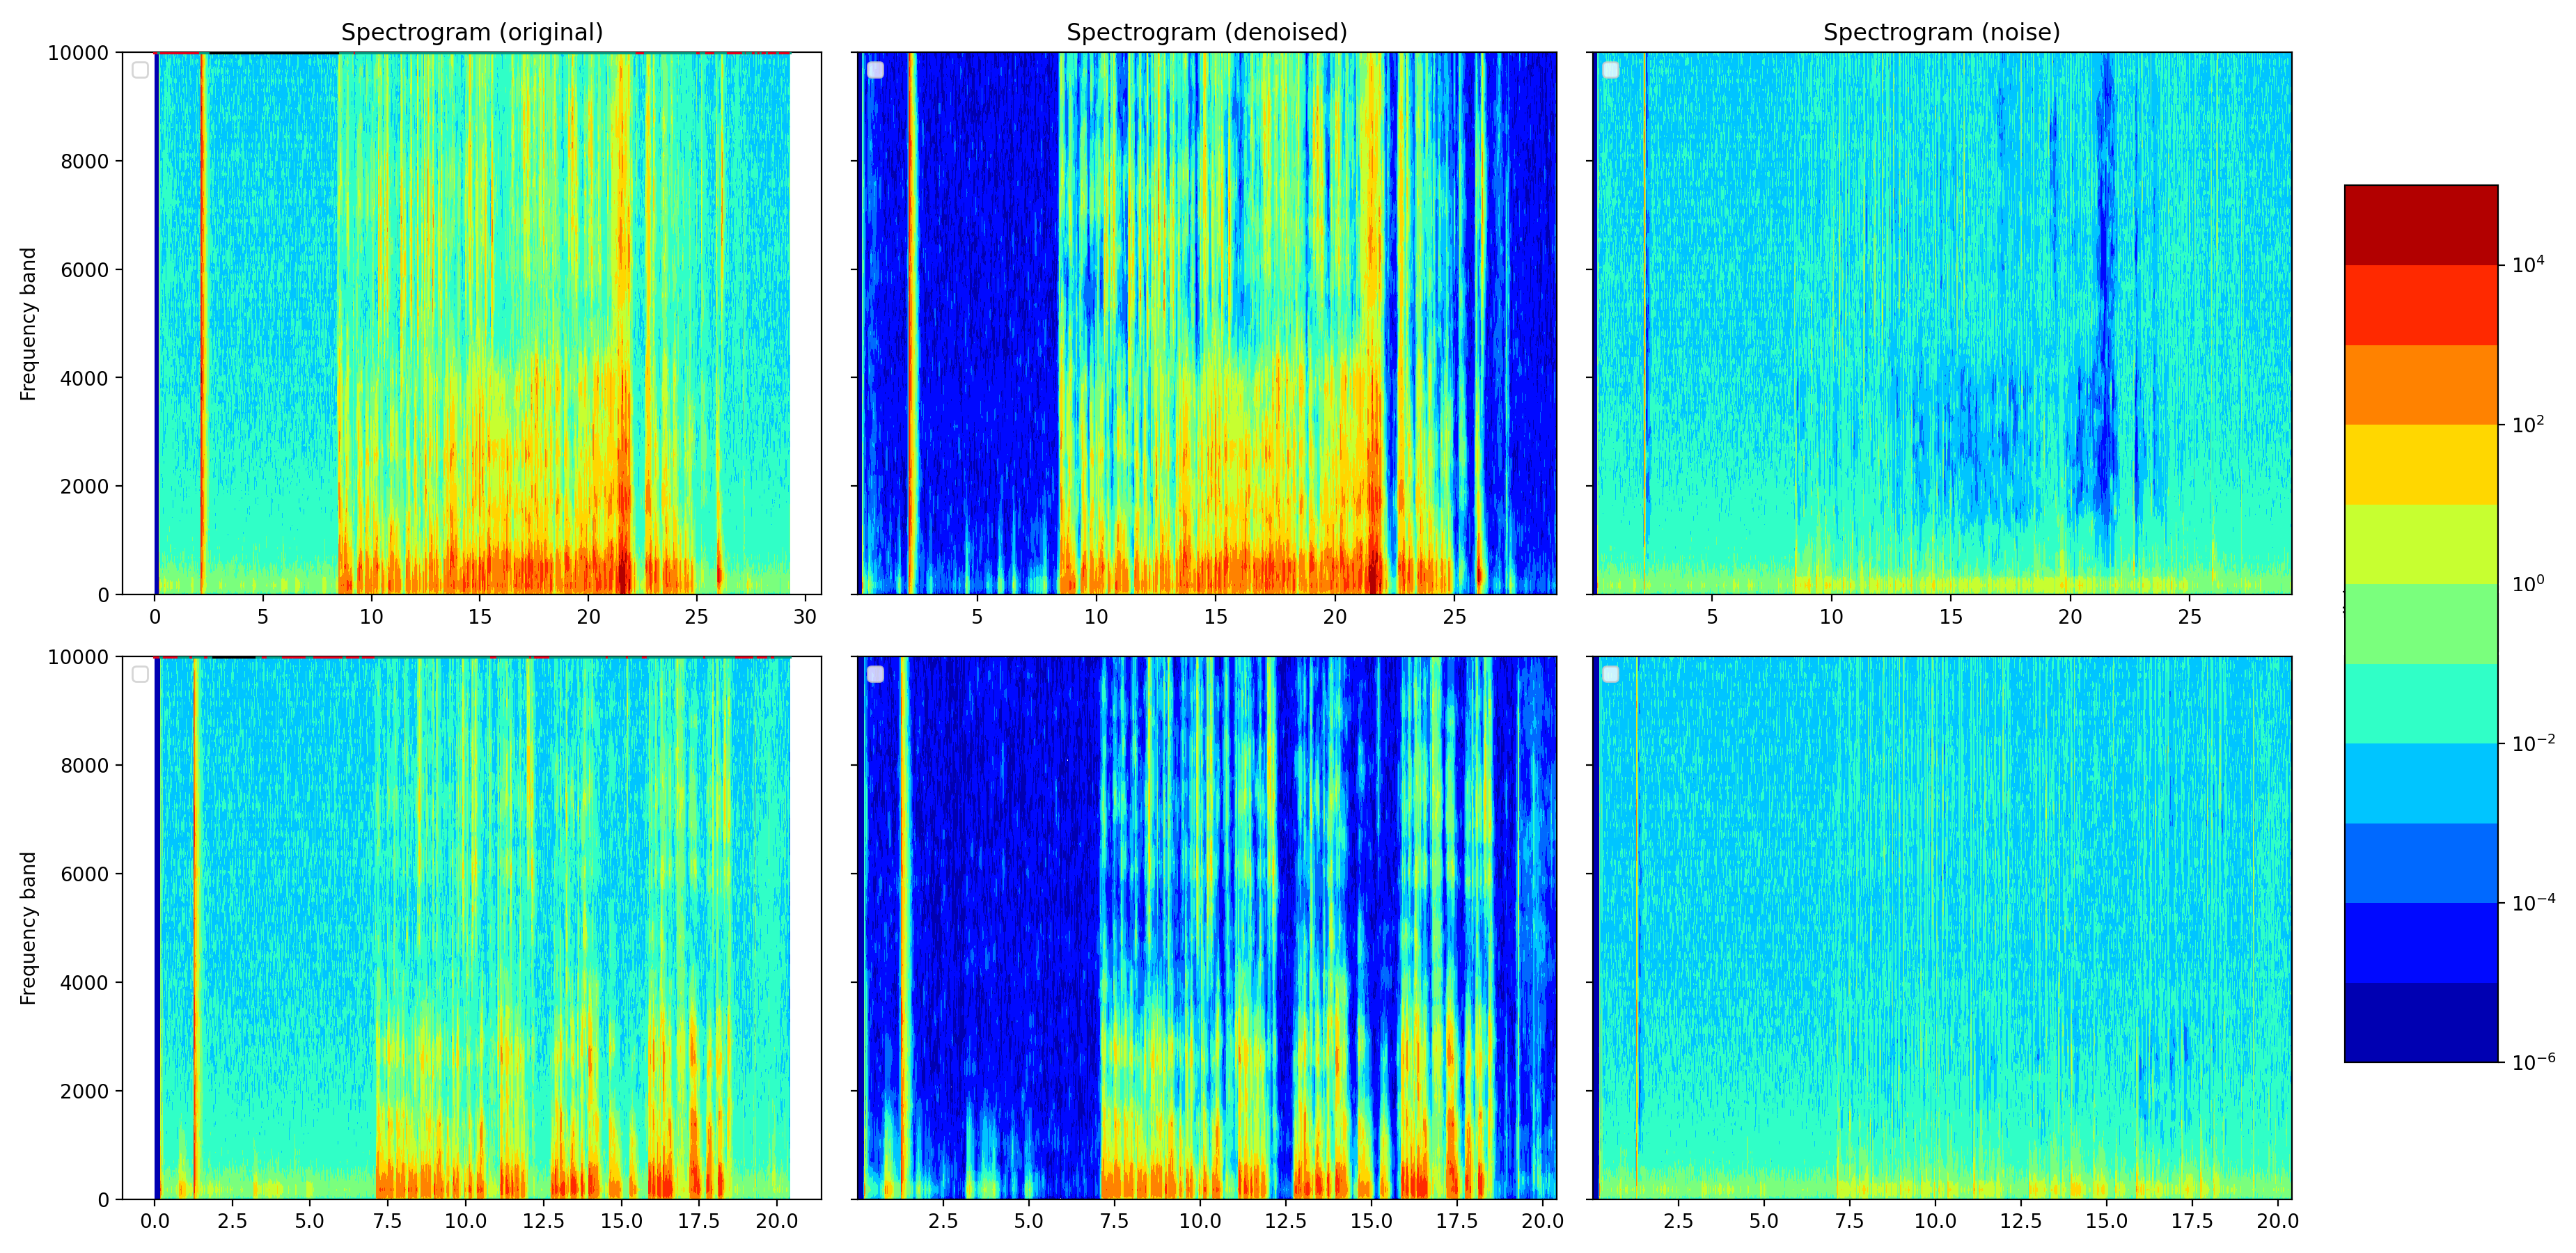
\includegraphics[width=1.0\textwidth]{media/denoiser2mp}
	\caption{Darstellung der Rauschextraktion von zwei Aufnahmen (obere bzw. untere Zeile) aus der Umgebung „Raum 2“. Es handelt sich jeweils um Zeit-Frequenzplots bei denen die Farben das jeweilige Energielevel der entsprechenden Frequenz zum entsprechenden Zeitpunkt darstellen. Von links nach rechts sind jeweils erst Originaldaten, dann das rauschreduzierte Signal und schließlich das reine Rauschen nach Multiband Spectral Subtraction dargestellt. Auf der x-Achse sind jeweils Sekunden, auf der y-Achse Hertz aufgetragen.}
	\label{fig:denoise}
\end{figure}

Um mehr Informationen über die erste Stufe der Rauschdetektion zu erhalten, ist in den linken Plots von Abbildung~\ref{fig:denoise} und allen Plots von Abbildung~\ref{fig:compare} die Klassifizierung in Sprache und reines Rauschen oben mit dünnen Stricken farblich dargestellt. Dabei stellt grün Sprachsequenzen, rot reines Rauschen und schwarz das längste, also zur weiteren Verarbeitung genutzte, Intervall reinen Rauschens dar. Mit kleinen Unterbrechungen entspricht dies weitgehend der intuitiven Klassifizierung anhand der akustischen Beurteilung und kann ansonsten auch in der Sensibilität angepasst werden. In der Umgebung „Platz“ sind die erkannten Rauschintervalle teils recht kurz, da starker Wind teilweise als Sprache klassifiziert wurde. In Tests mit einem anderen Aufnahmegerät funktionierte die Zuordnung teils schlechter und klassifizierte zu oft als Sprache, was zu wenig reinen Rauschintervallen führte. Erklärt werden kann dies unter Umständen mit einem dort aktivierten Software-Rauschfilter, der zu unreinen Audiosignalen führte.

Als nächstes betrachten wir nun also die Rauschsignale verschiedener Aufnahmen an verschiedenen Umgebungen in Abbildung~\ref{fig:compare}. Teilweise sind in diesen Plots in den Spalten stärkere Gemeinsamkeiten erkennbar, die für die spätere Klassifizierung vielversprechend sind. Teilweise wirken die Spektrogramme verschiedener Orte allerdings auch sehr ähnlich und weisen auch innerhalb der Spalten Abweichungen auf. Wie zu erwarten, sind sich beispielsweise die Umgebungen „Raum~1“ und „Raum~2“ recht ähnlich. Akustisch sind diese ebenfalls nicht zu unterscheiden, die Umgebungen „Platz“ (durch starken Wind) und „Straße“ (durch lokalen Geräuschanstieg durch Autos) heben sich akustisch noch meist ab.

\begin{figure}[h]
	\centering
	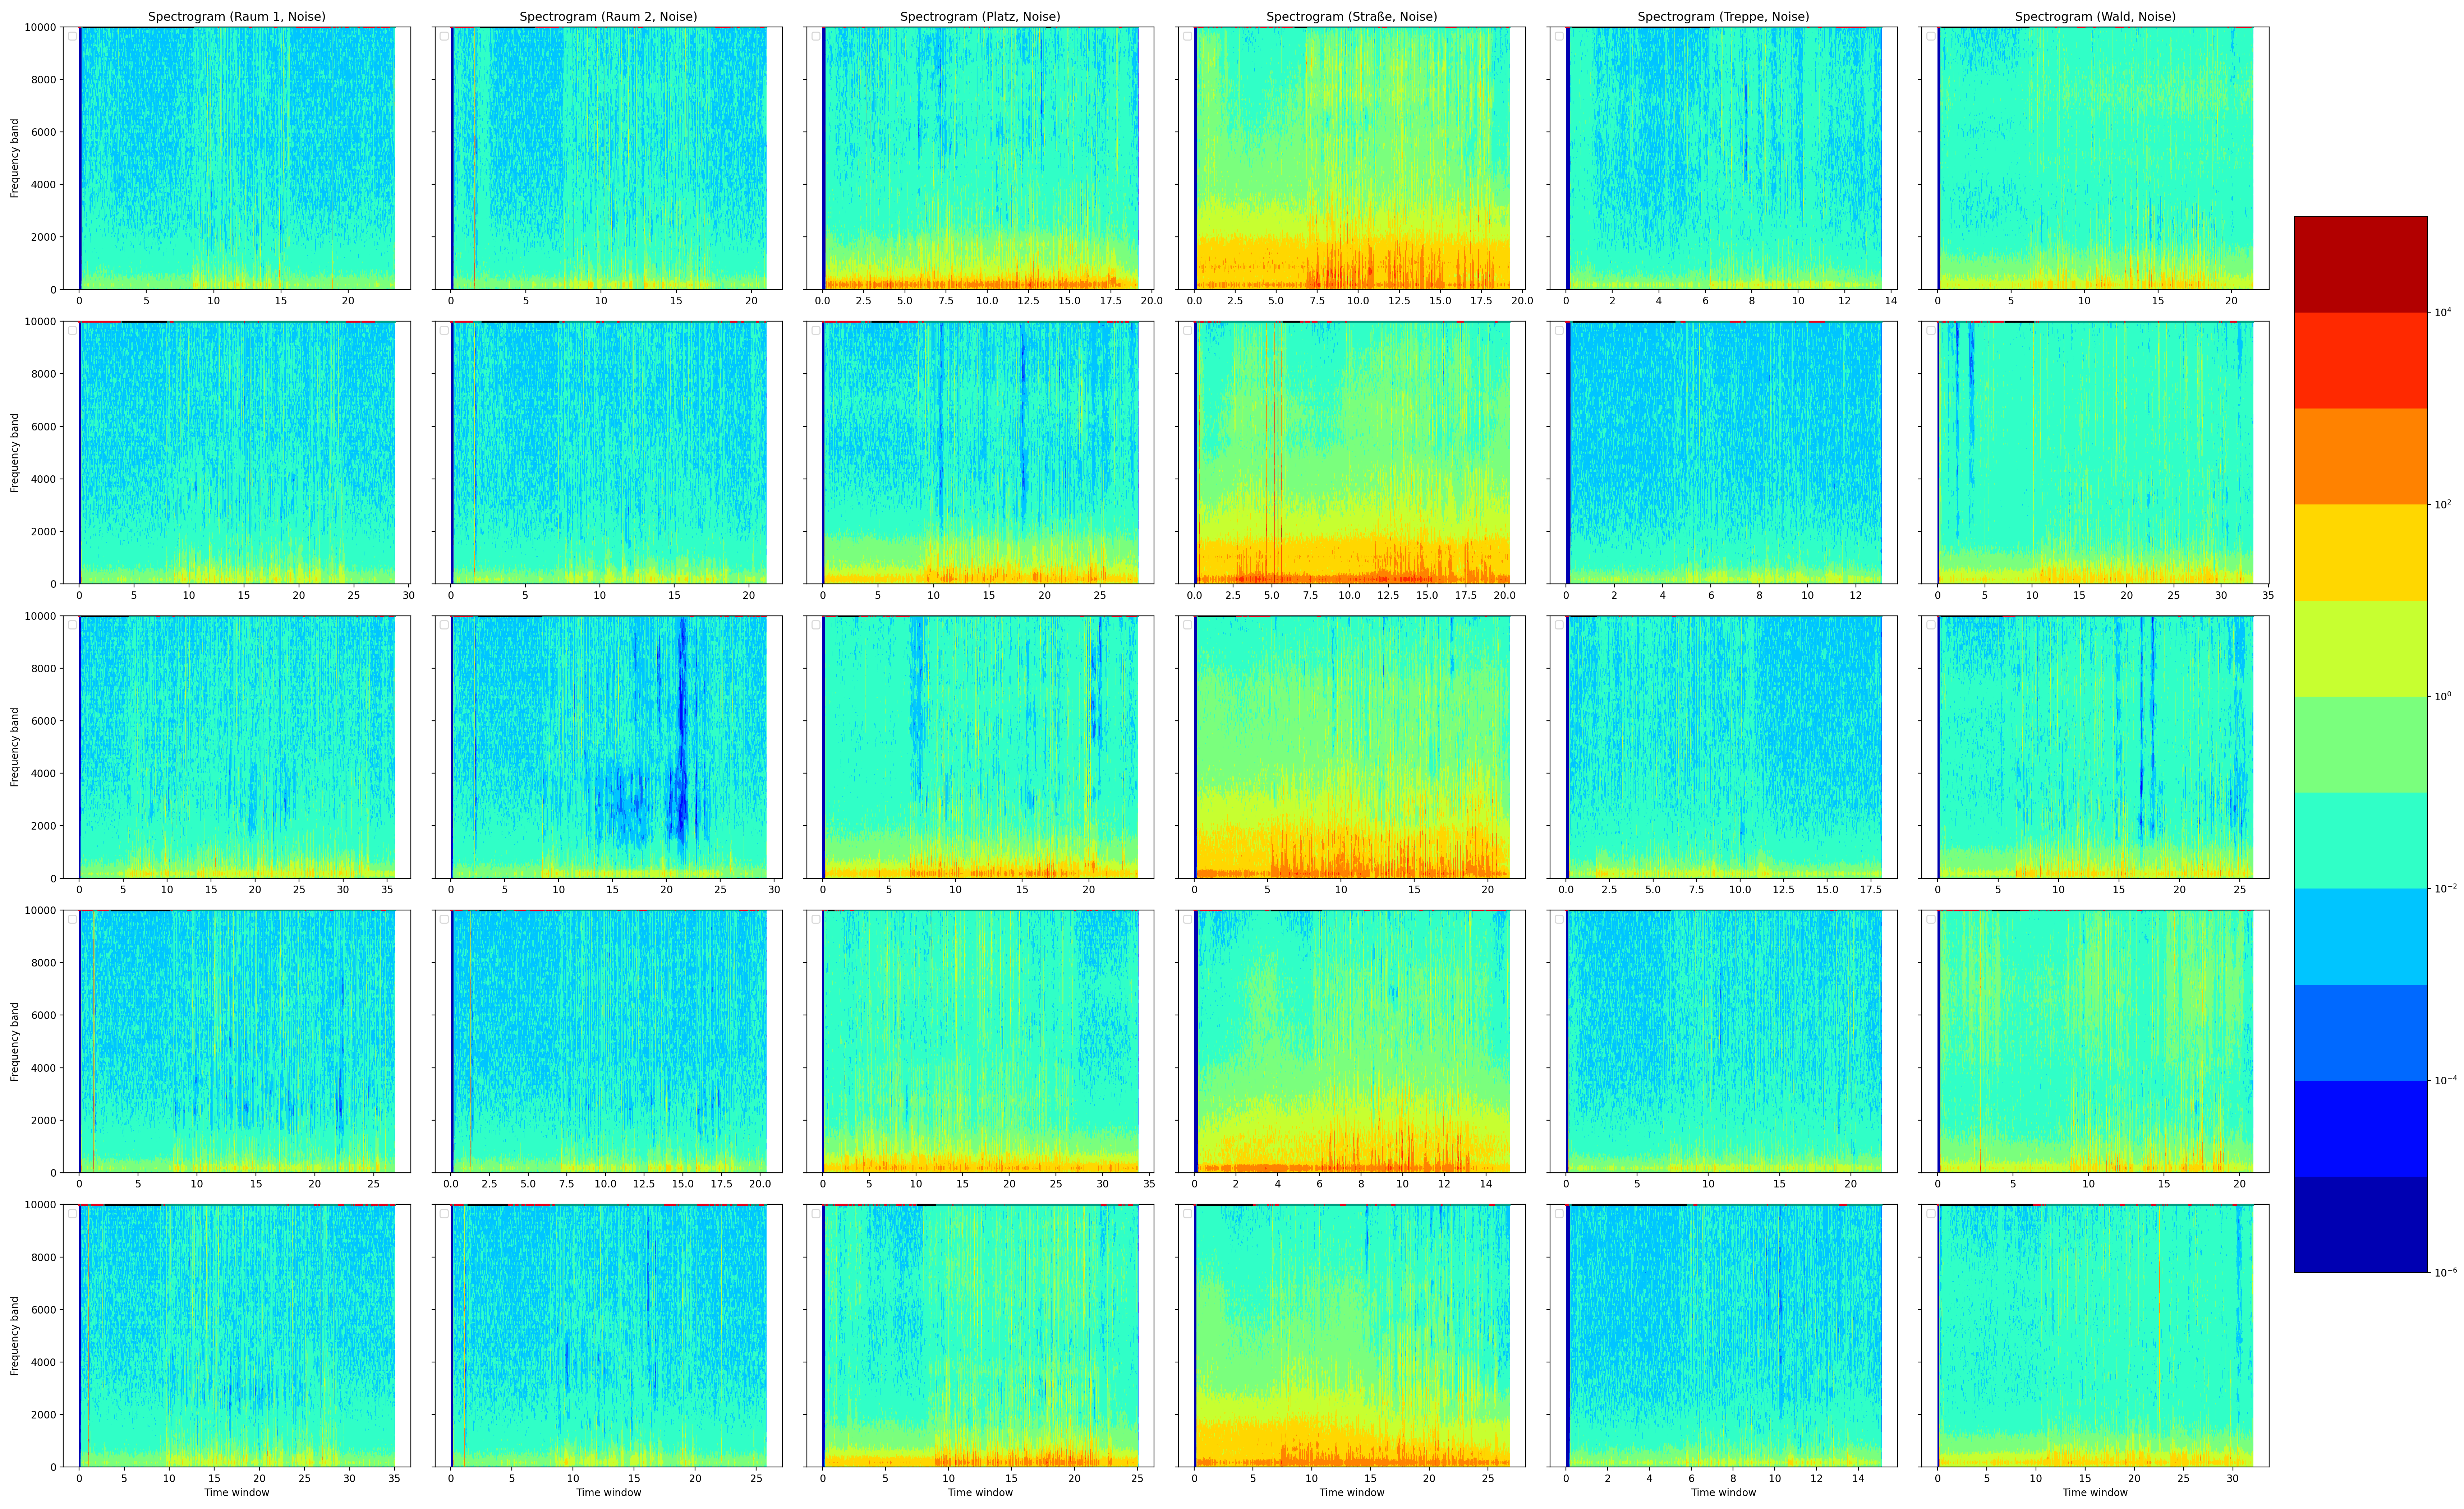
\includegraphics[width=1.0\textwidth]{media/comp}
	\caption{Darstellung der Rauschapproximationen verschiedener Aufnahmen (Spalten sind Umgebungen, Zeilen verschiedene dort aufgenommene Aufnahmen). Es handelt sich jeweils um Zeit-Frequenzplots bei denen die Farben das jeweilige Energielevel der entsprechenden Frequenz zum entsprechenden Zeitpunkt darstellen. Die Multiband Spectral Subtraction war hier deaktiviert, da die Unterschiede dadurch optisch besser erkennbar sind. Auf der x-Achse sind jeweils Sekunden, auf der y-Achse Hertz aufgetragen.}
	\label{fig:compare}
\end{figure}

Schließlich wenden wir uns noch dem Vergleich der Umgebungs-Rauschapproximationen zu. Um die Umgebungen zu vergleichen, haben wir für jede dieser Umgebungen einen Vektor von Energie in verschiedenen Frequenzbändern (vgl. Abschnitt \ref{envdetect}). Dieser ist in Abbildung~\ref{fig:envs} für unsere Umgebungen dargestellt. Die Umgebung „Straße“ hebt sich hier schon durch hohe Intensität deutlich ab. „Platz“ und „Wald“ haben jeweils ein Maximum um $7\cdot10^3$~Hz, unterschieden sich aber auch im Verlauf in Richtung niedriger Frequenzen. Die drei verbleibenden und im gleichen Haus aufgenommenen Aufnahmen unterscheiden sich hingegen weniger deutlich. Hier zeichnen sich Schwierigkeiten bei der Klassifizierung der Aufnahmen ab.

\begin{figure}[h]
	\centering
	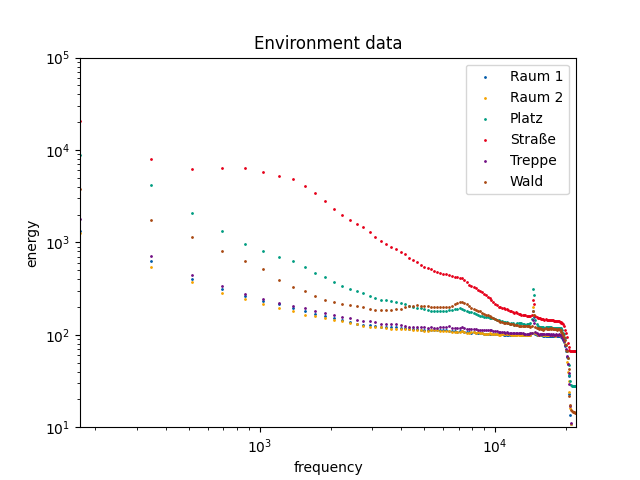
\includegraphics[width=0.45\textwidth]{media/envs}
	\caption{Darstellung der Rauschapproximationen verschiedener Umgebungen (eine Farbe pro Umgebung). Es handelt sich um einen Frequenz-Intensitätsplot. Die Multiband Spectral Subtraction war hier deaktiviert, die Unterschiede zu aktivierter Multiband Spectral Subtraction sind nicht groß. Auf der x-Achse sind Hertz aufgetragen.}
	\label{fig:envs}
\end{figure}

In allen Graphen ist ein starker Abfall der Intensitäten in hohen Frequenzen zu verzeichnen, der sowohl durch wenig akustischen Signalen in diesem Bereich als auch durch Schwächen des Aufnahmegerätes erklärbar ist. Außerdem haben alle Umgebungen einen starken punktuellen Anstieg bei etwa $1,5\cdot10^4$~Hz. Da dieser bei Referenzaufnahmen mit anderen Geräten nicht auftritt, ist dies sicherlich auf eine Schwäche des Aufnahmegeräts, beispielsweise durch eine Eigenfrequenz zurückzuführen.

Bei Betrachtung der Unterschiede zwischen den einzelnen Aufnahmen einer Umgebung (Abbildung~\ref{fig:envs2}) stellen wir fest, dass auch hier Unterschiede erkennbar sind, diese jedoch in den meisten Fällen geringer ausfallen, als die zwischen den Umgebungen. Eine Unterscheidung der Räume und des Treppenhauses scheint weiterhin schwierig, da die Abweichungen zwischen diesen Abweichungen die Differenzen aus Abbildung~\ref{fig:envs} zu übersteigen scheinen.

\begin{figure}[h]
	\centering
	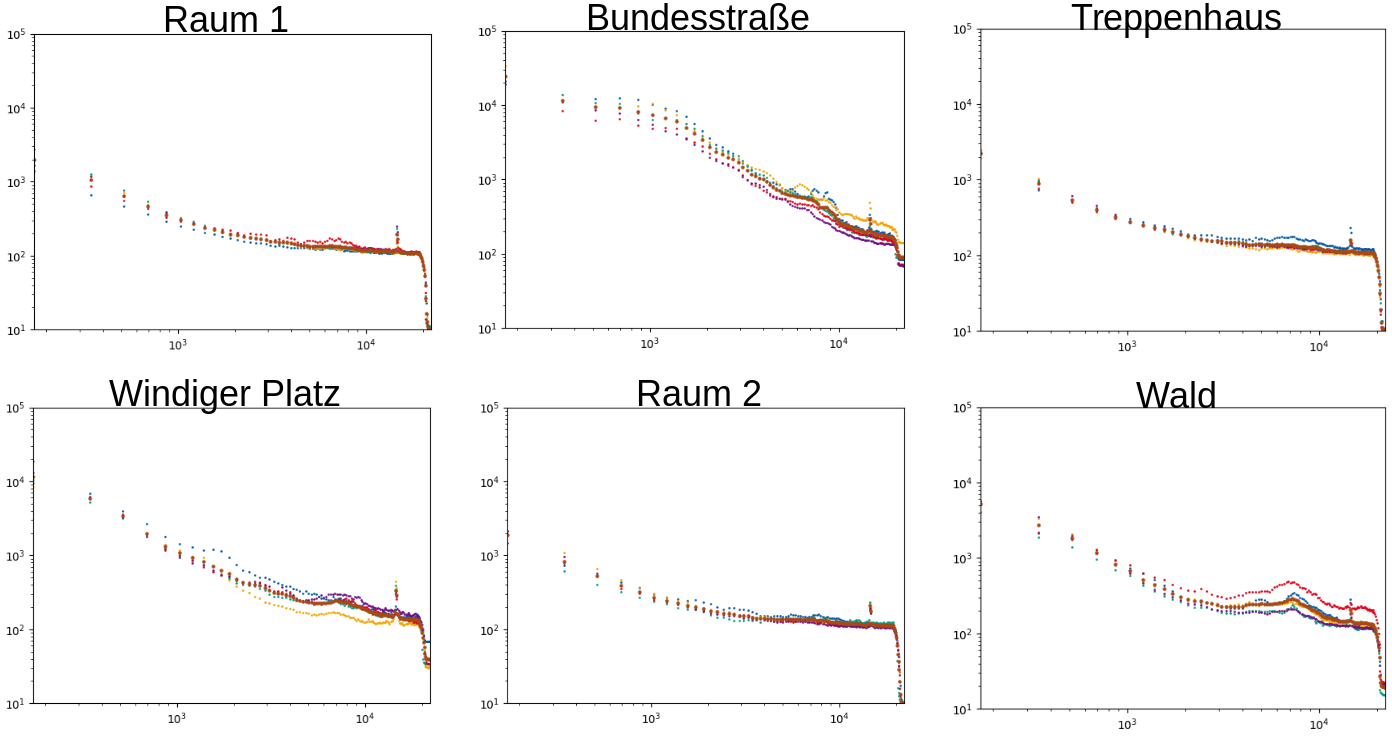
\includegraphics[width=0.75\textwidth]{media/envs2}
	\caption{Darstellung der Rauschapproximationen der einzelnen Aufnahmen der Umgebungen (eine Farbe pro Aufnahme). Es handelt sich um Frequenz-Intensitätsplots. Auf den x-Achsen sind Hertz aufgetragen.}
	\label{fig:envs2}
\end{figure}



\pagebreak
\subsection{Erkennung}
\label{erkennung}

Zum Test der Umgebungserkennung haben wir die aus den Umgebungen aus Abschnitt \ref{envs} generierten Rauschapproximationen erstellt. Zunächst versuchen wir nun die einzelnen dieser Aufnahmen den Umgebungen wieder zuzuordnen\footnote{Hierbei sind die zuzuordnenden Testdaten auch in der Umgebungsgenerierung genutzt worden. Durch die vorherige Median-Bildung über die Werte aller Fenster in allen dort aufgenommenen Aufnahmen, gehen wir jedoch davon aus, dass die Ergebnisverfälschung dadurch gering ist. Tests bei denen nur auf den anderen Aufnahmen des Ortes die Umgebung generiert wurde oder neue Aufnahmen zugeordnet wurden, führten zu ähnlichen Ergebnissen.}. Die Ergebnisse unterscheiden sich mit den verschiedenen in Abschnitt~\ref{envdetect} beschriebenen Parametern, zwei gute Ergebnisse sind in Abbildung~\ref{fig:vals1} dargestellt. Im linken Beisiel wurden einige Umgebungen richtig erkannt. Vor allem wurden jedoch einige in „Raum 1“ aufgenommene Aufnahmen zu „Raum 2“ zugeordnet was aufgrund der ähnlichen Eigenschaften der Räume wenig überraschend ist. Im rechten Beispiel funktioniert die Klassifizierung der beiden Räume etwas besser, dafür gibt es im Treppenhaus einige Fehlklassifizierungen. Die verschiedenen Parameter erzielen an verschiedenen Stellen also unterschiedlich gute Ergebnisse. Bei Fehlklassifizierungen sind die richtigen Umgebungen jedoch meist noch grün was eine immer noch geringe Abweichung (also kleine Zahl) darstellt.

\begin{figure}[ht]
	\centering
	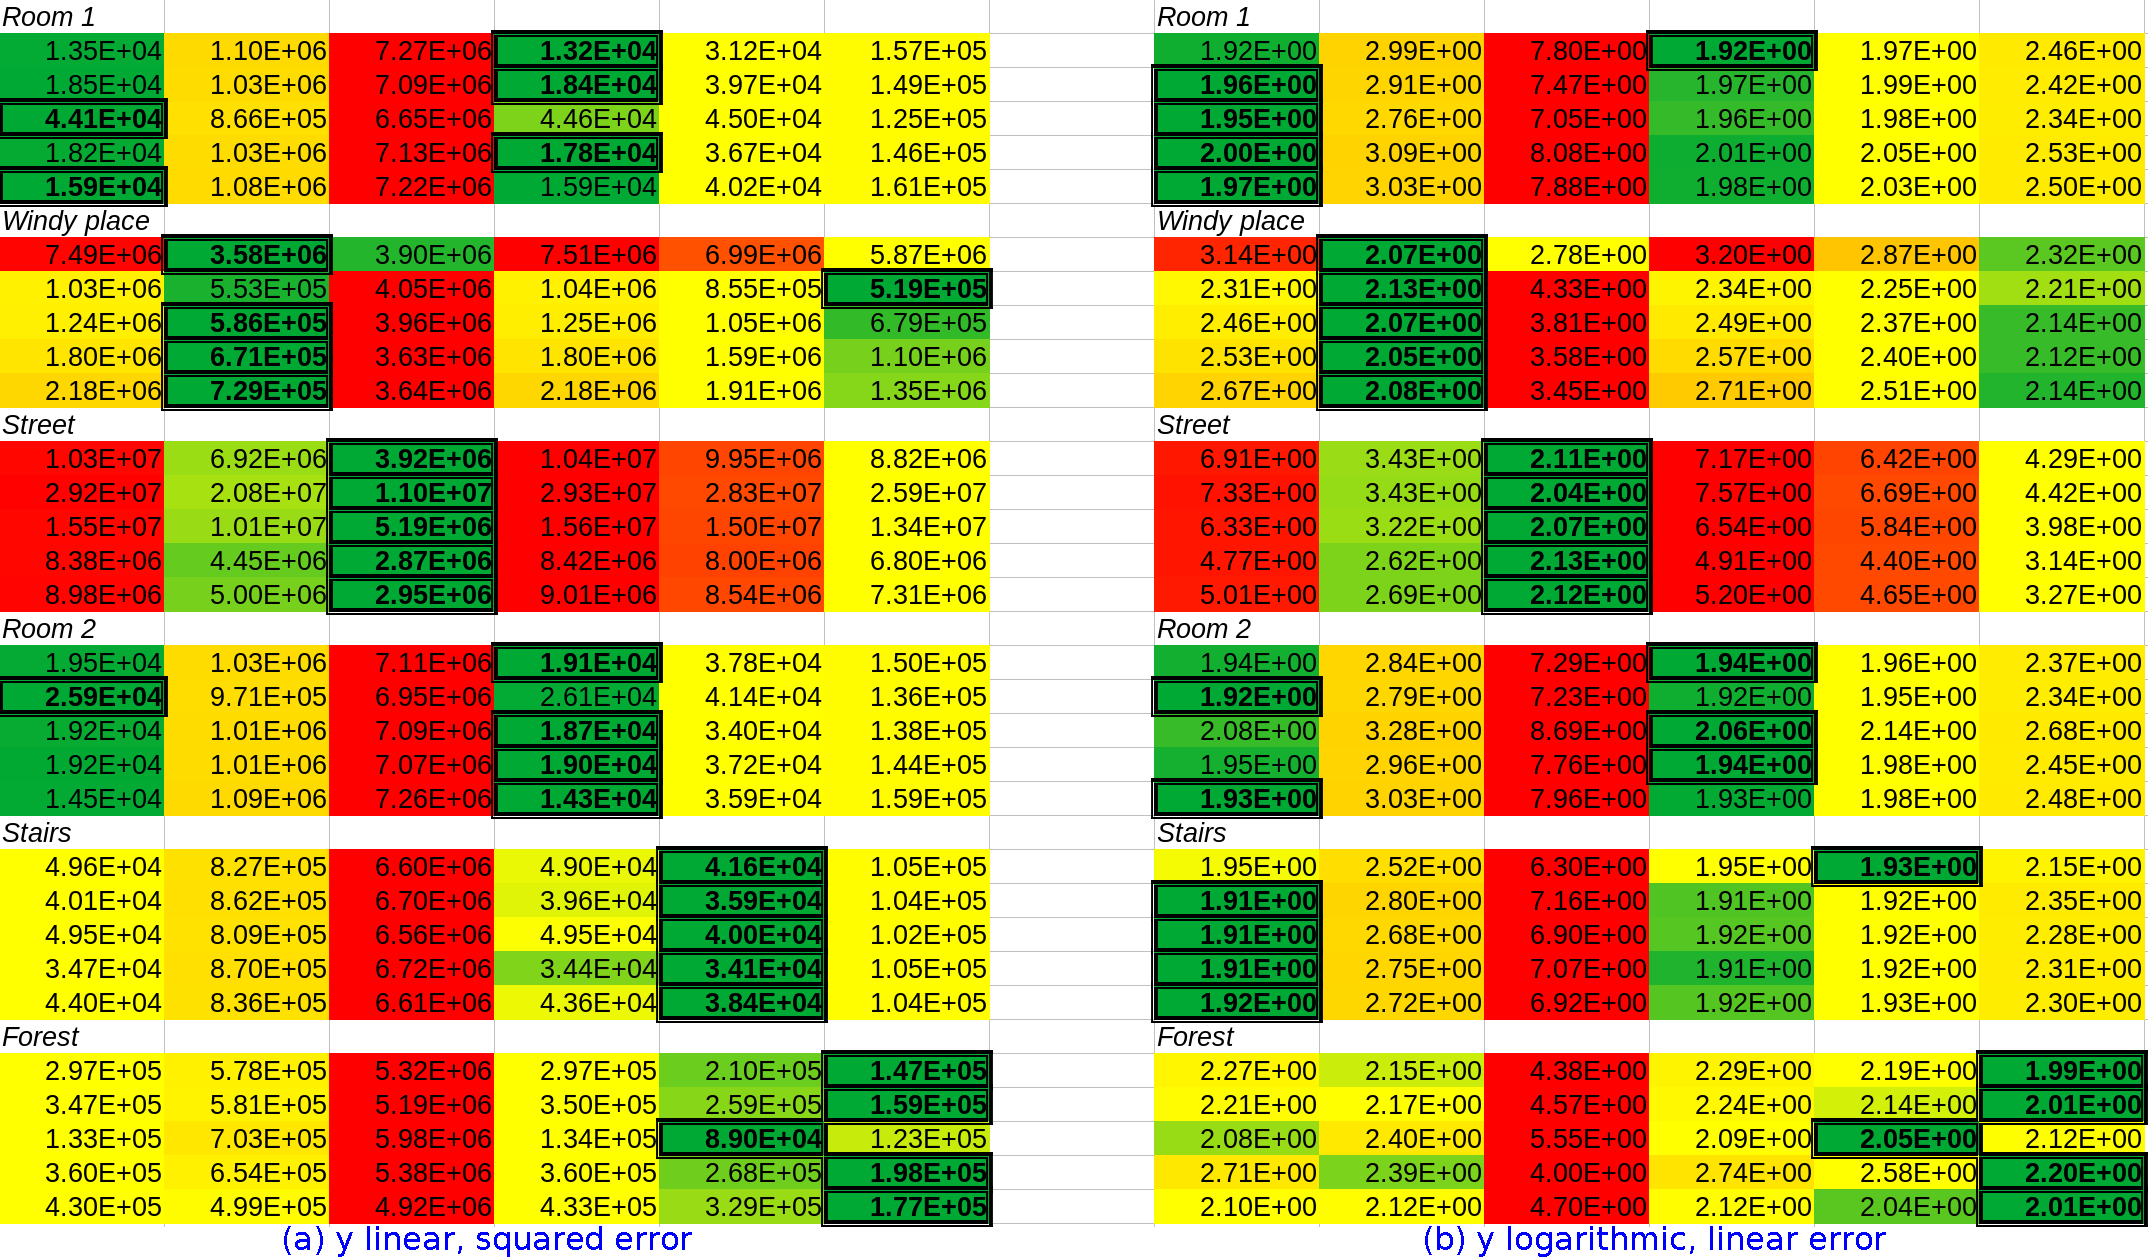
\includegraphics[width=1.0\textwidth]{media/vals2}
	\caption{Ergebnis der Umgebungserkennung auf den verschiedenen Audiodateien. Links wurden die Standardparamter aus Abschnitt~\ref{envdetect} genutzt, rechts wurde eine lineare Abweichungsberechnung und eine logarithmische y-Skalierung genutzt. Pro Zeile sind jeweils die Werte einer Aufnahme angegeben, die Umgebung der folgenden 5 Aufnahmen ist jeweils über den Blöcken angegeben. In den Spalten sind jeweils die Abweichungswerte zu den einzelnen Umgebungen dargestellt, die Umgebungen sind hier in der gleichen Reihenfolge wie der der Blöcke dargestellt. Kleine Zahlen entsprechen einer höheren Wahrscheinlichkeit, dass diese Umgebung die der Aufnahme war, die wahrscheinlichste Umgebung ist jeweils eingerahmt. Optimal wären die eingerahmten Einträge im $n$-ten Block in der $n$-ten Spalte.}
	\label{fig:vals1}
\end{figure}

Um die Störabweichung zu untersuchen haben wir in „Raum 2“ jeweils zwei Aufnahmen mit unter der Bettdecke liegendem Mobiltelefon, bei geöffneten Fenster und mit den alten Bedingungen gemacht. Die Rauschapproximation der Umgebung basiert weiterhin auf den alten Aufnahmen. Die Ergebnisse sind in Abbildung~\ref{fig:vals2} dargestellt. Dabei wurde die Aufnahmen unter der Bettdecke und die unter den alten Bedingungen korrekt zugeordnet. Bei geöffnetem Fesnter wurden die Aufnahmen der Umgebung „Treppenhaus“ zugeordnet. Da diese jedoch bei geöffnetem Fenster im gleichen Gebäude aufgenommen wurde, ist dieses Resultat jedoch nicht überraschend.

\begin{figure}[h]
	\centering
	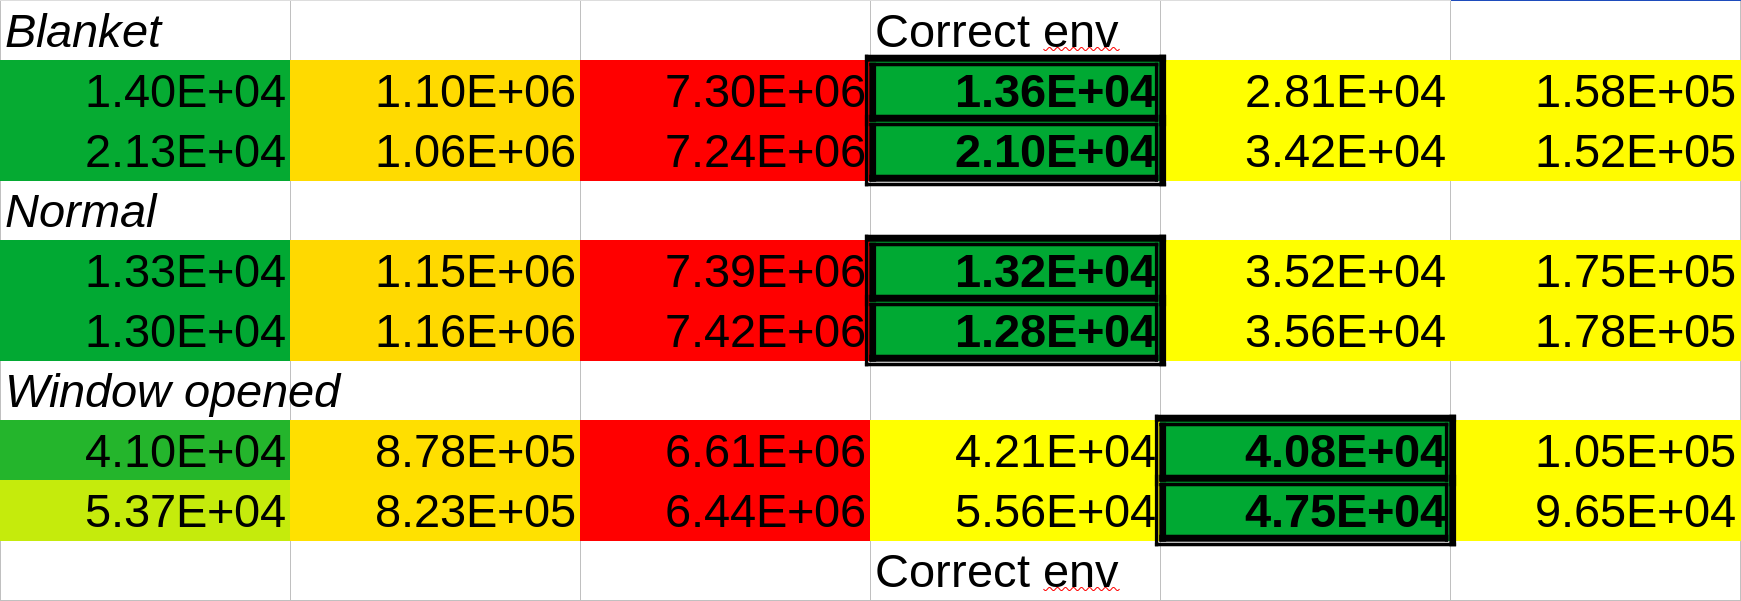
\includegraphics[width=0.5\textwidth]{media/vals1}
	\caption{Ergebnis der Umgebungserkennung auf den verschiedenen Audiodateien. Pro Zeile sind jeweils die Werte einer Aufnahme angegeben, die Eigenschaften der folgenden 2 Aufnahmen ist jeweils über den Blöcken angegeben. In den Spalten sind jeweils die Abweichungswerte zu den einzelnen Umgebungen dargestellt, die Umgebungen sind hier wie in Abbildung~\ref{fig:vals1}. Kleine Zahlen entsprechen einer höheren Wahrscheinlichkeit, dass diese Umgebung die der Aufnahme war, die wahrscheinlichste Umgebung ist jeweils eingerahmt. Optimal wären eingerahmte Einträge in der $4$-ten Spalte („Raum 2“).}
	\label{fig:vals2}
\end{figure}


\IMRADlabel{discussion}
\subsection{Resümee}

Unsere Rauschextraktion macht es für menschliche Hörer*innen meist schwer noch Teile der Sprache zu verstehen bzw. erfordert dazu eine deutliche Verstärkung des Signals. Subjektiv wirkt die Rauschentfernung ohne aufwändige Konfiguration besser als die beispielsweise in Audacity \cite{audacity_audacity_nodate} implementierte was an flexiblerer Implementierung der genutzten Funktionen und der automatischen Detektion eines geeigneten Rauschintervalls liegen könnte. Die Multiband Spectral Subtraction führte zu weniger Voice Leakage, reduzierte aber auch die Gesamtenergie – insgesamt funktionierten die weiteren Funkionen unserer Software nach Anwendung von Multiband Spectral Subtraction nicht wesentlich besser.

Die Erkennung der Umgebungen funktioniert mit den meisten Parametern recht zuverlässig auf sehr unterschiedlichen Umgebungen, bei ähnlichen Umgebungen wie etwa den beiden benachbarten Räumen funktioniert sie teils nicht mehr oder nur mit wenigen Parametern.

Der Vergleich mit \cite{ikram_digital_2010} fällt schwer, da nach Rauschunterdrückung zwar ähnliche Plots zu Abbildung \ref{fig:denoise} angegeben werden, uns jedoch keine Audiodaten vorliegen. Aus den Plots gehen wir davon aus, dass die Ergebnisse unserer ähnlichen Rauschentfernungsansätze ähnlich gut sind. Die Umgebungserkennung ist schon bei leicht unterschiedlichen Aufnahmen kaum noch vergleichbar was eine Beurteilung der Unterschiede schwierig macht. Die Detektion von Manipulationen innerhalb einzelner Dateien ist bei uns derzeit nicht implementiert, siehe Abschnitt~\ref{manipulationdet}.



\pagebreak
\section{Mögliche Erweiterungen}
\label{future}

Hier werden ein paar Ideen zur Erweiterung und Verbesserung unserer Software kurz vorgestellt, die über den Rahmen dieses Praktikums hinausgehen.

\paragraph{Zeitliche Änderungen}
Viele Geräusche treten nicht dauerhaft sondern immer wieder kurz auf, beispielsweise vorbeifahrende Autos auf einer Bundesstraße. Diese werden durch die aktuelle Median-Bildung über den zeitlichen Verlauf nicht optimal abgebildet und könnten durch neue Ansätze besser in die Erkennung einbezogen werden.

\paragraph{Verschiedene Aufnahmegeräte}
Um Auswirkungen verschiedener Aufnahmegeräte besser analysieren zu können, müsste zunächst ein insgesamt niedrigeres Energielevel einer Aufnahme ausgeglichen werden, um nur relative Unterschiede zwischen den Frequenzbändern zu betrachten. Anschließend könnten durch weitere Maßnahmen mehr Verbesserungen zum Ausgleich aufnahmegerätabhängiger Effekte ergriffen werden, etwa ein Ausgleich der in Abbildung~\ref{fig:envs} festgestellten lokalen Ausreißer bei $1,5\cdot10^4$~Hz.

\paragraph{Grenzwert}
Die aktuelle Implementierung sucht nach der bestpassendsten aus mehreren bekannten Umgebungen. Wünschenswert wäre ein Plausibilitätswert für eine Umgebung, der von anderen Umgebungen unabhängig ist. Aktuell wäre ein solcher Wert stark von den Parametern abhängig, funktioniert aber auch nur begrenzt. Insgesamt ist hierzu vermutlich eine weitere Verfeinerung der Metrik mit neuen Ansätzen nötig.

\paragraph{Wahrscheinlichkeiten}
Beispielsweise um Grenzwerte zu realisieren, hätten wir gerne eine Wahrscheinlichkeitsverteilung, um Konfidenzintervalle anzugeben, in denen wir eine Aufnahme einer Umgebung zuordnen. Da wir durch die einzelnen Fenster viele Werte haben wie stark die einzelnen Frequenzen in einer Aufnahme enthalten sind, könnten wir diese als eine Gauß-Glocke pro Frequenz approximieren und anschließend Aufnahmen durch die Positionen in diesen Gauß-Glocken zuordnen. Da dieser Ansatz jedoch zunächst alle Frequenz-Intensitäten als unabhängig ansehen würde, müsste dieser mathematisch noch weiter entwickelt werden, um ihn einsatzbereit zu machen.

\paragraph{Manipulationserkennung}
\label{manipulationdet}

Neben der Abschätzung, ob eine Umgebung zu einer Aufnahme plausibel ist oder der Zuordnung von Aufnahmen zu Umgebungen ist auch die Erkennung von Schnitten bzw. Manipulationen in Aufnahmen auf Basis von Rauschen forensisch interessant. Für diese sind mehrere Ansätze denkbar.

\cite{ikram_digital_2010} untersucht die Ähnlichkeit von Gesamtaufnahmen zu verschiedenen Umgebungen und vermutet bei mehreren ähnlichen Umgebungen, dass Anteile beider Umgebungen enthalten sind. Dazu ist es in unserer Implementierung vermutlich nötig den Median über die Frequenzen der Fenster der Aufnahme durch einen Mittelwert zu ersetzen, um nicht kurze starke Abweichungen direkt zu eliminieren. Der Ansatz hat jedoch die Nachteile, dass die potenzielle Umgebung einer Manipulation bekannt sein muss und die Tests funktionierten nachdem dort recht große Anteile hineinkopiert wurden. Bei kurzen manipulierten Stellen, könnte das deutlich schlechter funktionieren.

Ein weiterer Ansatz wäre starke Abweichungen zwischen verschiedenen, kurzen Fenstern zu untersuchen und Manipulationen zu vermuten, wenn ein oder mehrere benachbarte Fenster stark von den übrigen Fenstern abweichen. Dieser Ansatz könnte jedoch auch bei verbleibender Voice Leakage, also übrigen Sprachanteilen oder zu stark reduzierter Sprache eine Manipulation vermuten.

\pagebreak

\section{Bedienung}
\label{usage}


\subsection{Einrichtung}

\begin{enumerate}
	\item Erstellen Sie eine virtuelle Umgebung mit dem Befehl \texttt{virtualenv \$name}
	\item Aktivieren Sie diese mit \texttt{source \$name/bin/activate}
	\item Installieren Sie alle erforderlichen Pakete mit \texttt{pip install -r requirements.txt}.
\end{enumerate}

Nach Änderung des Codes müssen die erforderlichen pakete ggf. durch \texttt{pip freeze > requirements.txt} angepasst werdenx

\subsection{Ausführung}

Durch Ausführen von \texttt{python main.py} im Ordner \texttt{src} wird der Code ausgeführt. Dazu müssen vorher die Paramter angepasst werden und ggf. die benötigten Audiodateien entsprechend der Parameter und Ordnerstruktur hinterlegt werden.

Ein Beispielskript zur Ausführung unter Linux wird bereitgestellt.

\subsection{Ordnerstruktur}

Es gibt die folgenden Ordner:

\texttt{src}: Hier liegt der Quellcode inklusive der \texttt{main.py}.

\texttt{Audio}: Hier liegen die einzugebenden Audiodateien.

\texttt{results}: Hier werden nach Ausführung der Software alle erstellten Dateien abgelegt. Dazu wird für jede Ausführung ein neuer Ordner mit der Run-ID (aufsteigende Zahlen) angelegt. In diesen liegen dann die Plots/Spektrogramme und Ausgabewerte (CSV), sowie Log-Dateien und Konfigurationsinformationen. Für die Audiodateien wird lediglich ein Pfad auf den Ordner \texttt{\_resources} in der Datei \texttt{run.js} angegeben, damit identische Dateien aus mehreren Ausführungen nicht mehrfach abgelegt werden.

\texttt{results}: Hier liegt die Projektdokumentation sowie eine Visualisierungsvorlage.

\subsection{Parametrisierung}
In der Datei \texttt{src/main.py}, können Funktionalitäten (de-)aktiviert werden und Parameter, wie bspw. die zu verarbeitenden Audiodateien) gesetzt werden. Im Code sind kurze Beschreibungen der einzelnen Einstellungen gegeben.

\paragraph{Audio} (Code-Kommentar „\texttt{Comparision metric parameters}“): Hier werden die Audiodateien festgelegt. Dazu gibt es ein Mapping von bekannten Umgebungen zu den dort erstellten Aufnahmen. Anschließend können weitere Aufnahmen festgelegt werden, die nun (so wie auch die Dateien zur Umgebungsgenerierung) den Umgebungen zugeordnet werden. Außerdem kann die Generierung von Audiodateien (ohne Rauschen / reines Rauschen) (de-)aktiviert werden.

\paragraph{Plots} (Code-Kommentar „\texttt{Graph properties}“): Hier können Einstellungen zu den Grafiken festgelegt werden, also bspw. Dateinamen, Aktivierung des Multipass-Ansatzes usw.

\paragraph{Metriken} (Code-Kommentar „\texttt{Comparision metric parameters}“): Die in Abschnitt \ref{envdetect} genannten Metrikanpassungen können eingestellt werden.

\subsection{Interpretation} 

Da auf die meisten Ausgabedaten schon in der Dokumentation näher eingegangen wurde, konzentrieren wir uns hier auf die numerischen Ergebnisse in der Datei \texttt{environment\_errors.csv} in den Ergebnissen. Hier stellen die Zeilen die zuzuordnenden Dateien dar und die jeweils kleinste Zahl entspricht der wahrscheinlichsten Umgebung für die Datei (s. Abschnitt~\ref{erkennung} für mehr Details). Mehrere kleine Zahlen zeigen weitere wahrscheinliche Umgebungen auf oder deuten auf Audioanteile beider Umgebungen in der Datei hin. Zur Visualisierung entsprechend Abbildung~\ref{fig:vals1} können die Werte in die Vorlage in \texttt{docs/data\_visualization\_template.ots} kopiert werden.

\appendix




\pagebreak
\printbibliography


%\affidavit



\end{document}
